% !TEX root = ../main.tex
\section{What is a Domain-Specific Language (DSL)?}

\subsection{The Core Idea}

A \textbf{domain-specific language} (DSL) is a programming language built for one thing.
Not a general tool, a scalpel. You trade the ability to do \emph{anything} for the
ability to express things in a specific domain so naturally that the program almost reads
like plain text written by a domain expert.

The observation that motivates DSLs is simple: every domain already has its own vocabulary.
Athletes talk about threshold runs and recovery swims. Database engineers talk about joins
and filters. Configuration engineers talk about rules and targets. When we force these people
to express their intent in a general-purpose language, we're adding a translation step that
doesn't need to exist. A DSL removes that step.

This is the trade-off at the core of every DSL:
\begin{center}
\textit{Turing-completeness} \quad for \quad \textit{domain clarity}
\end{center}

Most DSLs are not Turing-complete. That's a feature, not a limitation. A restricted
language can be analyzed, validated, and optimized in ways that a general-purpose language
cannot, precisely because it does less.

\subsection{Examples Worth Studying}

\subsubsection{SQL The Canonical DSL}

SQL is probably the most successful DSL ever written. The domain is relational data, and
the language maps almost perfectly onto how people think about tables and relationships.
Instead of writing a join algorithm, you write:

\begin{lstlisting}[language=SQL]
SELECT athlete.name, workout.distance
FROM athlete
JOIN workout ON athlete.id = workout.athlete_id
WHERE workout.date = '2026-05-03';
\end{lstlisting}

Notice what's missing; no loops, no memory management, no iteration order. The \emph{how}
(hash join? nested loop? index scan?) is the engine's problem. You only say \emph{what}
you want. That declarative gap between intent and execution is exactly what makes SQL so
readable decades after it was designed.

\subsubsection{Makefile: Dependency-Driven Computation}

A Makefile is a DSL for build systems. The domain is dependency graphs: given a set of
files and the commands that produce them, figure out the minimal set of steps needed to
bring everything up to date.

\begin{lstlisting}
main: main.o utils.o
	gcc -o main main.o utils.o

main.o: main.c defs.h
	gcc -c main.c

utils.o: utils.c defs.h
	gcc -c utils.c

clean:
	rm -f *.o main
\end{lstlisting}

The interesting thing about Makefiles is that the semantics are \emph{graph-based}: the
language describes nodes and edges, and the interpreter does a topological sort to figure
out what to run. Execution is lazy, nothing is rebuilt unless its dependencies changed.
This is very different from the imperative ``run these commands in order'' style of a shell
script. The DSL encodes the \emph{structure} of the computation, not the sequence.

\subsubsection{Regular Expressions Extremely Small Domain}

A regex like \texttt{[A-Z][a-z]+\textbackslash{}d\{4\}} replaces what would be
20--30 lines of character-matching code in a general-purpose language. The domain is so
narrow (string patterns) that you can pack enormous expressiveness into a handful of
characters. The downside is the flip side of that density: regexes are hard to read for
anyone who doesn't already speak the notation. This is a real design tension; concise
is not always readable.

\subsubsection{A Training DSL, the running example}

For this project, the domain is athletic training plans. A coach writing a plan might
naturally say ``Monday: threshold run, 10 kilometers, then 15 minutes of rest''. The
goal is to let them write something close to that:

\begin{lstlisting}
Monday:
  run: 10km @threshold
  rest: 15min

Wednesday:
  swim: 2000m steady
  strength: upper-body
\end{lstlisting}

This program is readable to a coach, unambiguous to a parser, and impossible to confuse
with anything other than a training plan. Compare it to the Python equivalent:

\begin{lstlisting}[language=Python]
plan.add_day("Monday", [
    Activity("run", distance=10, unit="km", intensity="threshold"),
    Activity("rest", duration=15, unit="min")
])
\end{lstlisting}

Both encode the same information. But the second one requires the coach to know Python,
understand objects and method calls, and care about quote marks and commas. The first
one doesn't. That's the whole point.

\subsection{A Formal Definition}

Formally, a DSL is a triple:
\[
  \text{DSL} = \langle \Sigma,\; \mathcal{G},\; \mathcal{S} \rangle
\]

where $\Sigma$ is the set of terminal symbols (the alphabet of the language), $\mathcal{G}$
is a grammar over $\Sigma$ that defines which strings are syntactically valid, and
$\mathcal{S}$ is a semantic function that maps parse trees to meanings. A program is any
string $p \in \mathcal{L}(\mathcal{G})$, and its meaning is $\mathcal{S}(\text{parse}(p))$.

This is the same structure as any programming language, the DSL isn't doing anything
fundamentally different from Python or Java at the formal level. The difference is in
scope: $\Sigma$ is small, $\mathcal{G}$ is simple, and $\mathcal{S}$ is restricted to
the domain.

\subsubsection{The Grammar in EBNF}

For the training DSL, a grammar in Extended Backus-Naur Form looks like this:

\begin{lstlisting}
plan      ::= day+
day       ::= DAY_NAME ':' NEWLINE activity+
activity  ::= EXERCISE ':' quantity intensity?
quantity  ::= NUMBER UNIT
intensity ::= '@' INTENSITY_LABEL

DAY_NAME  ::= 'Monday' | 'Tuesday' | ... | 'Sunday'
EXERCISE  ::= 'run' | 'swim' | 'cycle' | 'strength' | 'rest'
UNIT      ::= 'km' | 'm' | 'min' | 'h'
\end{lstlisting}

This grammar is context-free and unambiguous. It's small enough that a hand-written
recursive-descent parser can handle it in $O(n)$ time with just one token of lookahead.
That simplicity is intentional; if the grammar is getting complicated, it's usually a
sign that the language is trying to do too much.

\subsection{External vs Internal DSLs}

There are two main ways to build a DSL, and the choice has big consequences.

\subsubsection{External DSLs}

An external DSL is a standalone language. It has its own syntax, its own parser, and is
completely independent of any host language. SQL, Makefile, HTML, CSS, \LaTeX{}, and
Protocol Buffers are all external DSLs.

The upside is full control: the syntax can look exactly like the domain vocabulary, there
are no constraints from a host language, and non-programmers can read the programs.
The downside is real: you have to build everything yourself. Lexer, parser, semantic
analyzer, interpreter or compiler, error messages; all from scratch.

\subsubsection{Internal or Embedded DSLs}

An internal DSL lives inside a host language. It uses the host's features; method
chaining, operator overloading, macros, to approximate domain syntax while staying
legal in the host language:

\begin{lstlisting}[language=Python]
plan = (TrainingPlan()
    .on(Monday)
    .add_run(distance=10, unit='km', intensity='threshold')
    .add_rest(duration=15, unit='min'))
\end{lstlisting}

You get the host language's toolchain for free (parser, type checker, debugger, IDE
support). What you lose is syntax freedom, the result still looks like Python, and
errors still come from Python. For a training coach, this is probably a deal-breaker.
For a team of developers building a test framework (like pytest) or a query builder
(like SQLAlchemy), it's a perfectly good trade.

\subsubsection{The Decision}

The honest version of the trade-off is: if your users are domain experts who are
\emph{not} programmers, build an external DSL. If your users are developers who want
a cleaner API for a specific task, build an internal one.

\begin{center}
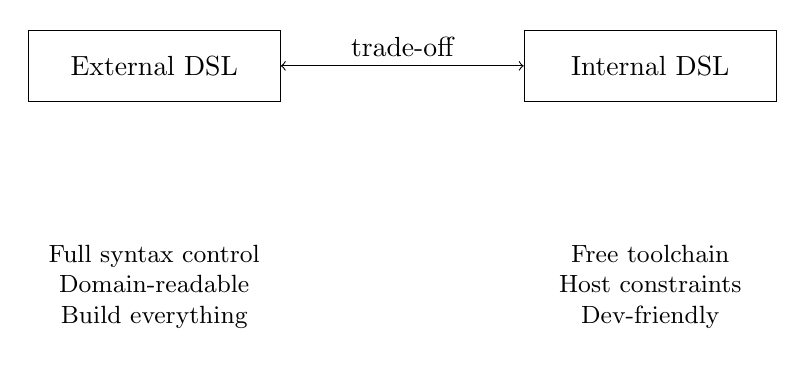
\begin{tikzpicture}[node distance=3.8cm]
  \node (ext) [draw, rectangle, minimum width=3.2cm, minimum height=0.9cm]
              {External DSL};
  \node (int) [draw, rectangle, minimum width=3.2cm, minimum height=0.9cm,
              right of=ext, xshift=2.5cm]
              {Internal DSL};
  \node (ext_d) [below of=ext, yshift=1cm, align=center, font=\small]
              {Full syntax control\\Domain-readable\\Build everything};
  \node (int_d) [below of=int, yshift=1cm, align=center, font=\small]
              {Free toolchain\\Host constraints\\Dev-friendly};
  \draw[<->] (ext) -- (int) node[midway, above] {trade-off};
\end{tikzpicture}
\end{center}

\subsection{How a DSL Program Gets Processed}

Every external DSL program goes through the same pipeline to become something executable.
Understanding this pipeline is important because most design decisions map directly to
one of these stages.

\begin{center}
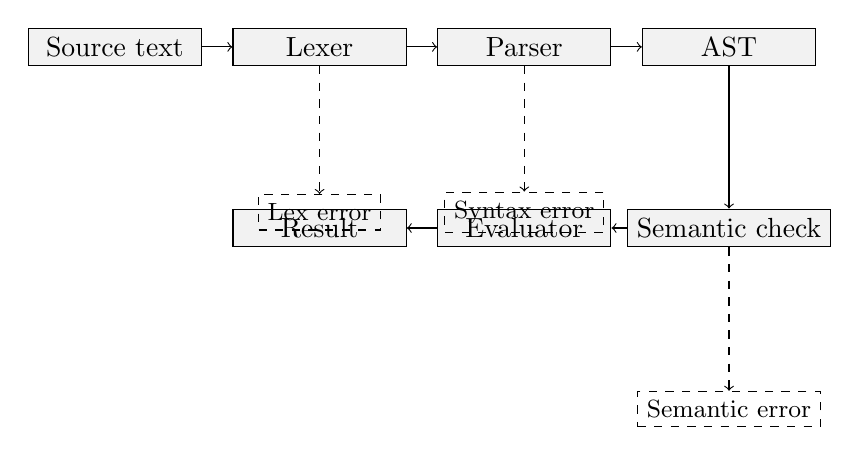
\begin{tikzpicture}[node distance=2.6cm]
  \node (src)   [draw, rectangle, fill=gray!10, minimum width=2.2cm]
                {Source text};
  \node (lex)   [draw, rectangle, fill=gray!10, minimum width=2.2cm,
                right of=src]
                {Lexer};
  \node (par)   [draw, rectangle, fill=gray!10, minimum width=2.2cm,
                right of=lex]
                {Parser};
  \node (ast)   [draw, rectangle, fill=gray!10, minimum width=2.2cm,
                right of=par]
                {AST};
  \node (sem)   [draw, rectangle, fill=gray!10, minimum width=2.2cm,
                below of=ast, yshift=0.3cm]
                {Semantic check};
  \node (eval)  [draw, rectangle, fill=gray!10, minimum width=2.2cm,
                left of=sem]
                {Evaluator};
  \node (out)   [draw, rectangle, fill=gray!10, minimum width=2.2cm,
                left of=eval]
                {Result};
  \node (err1)  [draw, rectangle, dashed, below of=lex, yshift=0.5cm,
                font=\small]
                {Lex error};
  \node (err2)  [draw, rectangle, dashed, below of=par, yshift=0.5cm,
                font=\small]
                {Syntax error};
  \node (err3)  [draw, rectangle, dashed, below of=sem, yshift=0.3cm,
                font=\small]
                {Semantic error};
  \draw[->] (src)  -- (lex);
  \draw[->] (lex)  -- (par);
  \draw[->] (par)  -- (ast);
  \draw[->] (ast)  -- (sem);
  \draw[->] (sem)  -- (eval);
  \draw[->] (eval) -- (out);
  \draw[->, dashed] (lex) -- (err1);
  \draw[->, dashed] (par) -- (err2);
  \draw[->, dashed] (sem) -- (err3);
\end{tikzpicture}
\end{center}

\begin{description}
  \item[Lexer] Takes the raw character stream and groups characters into tokens.
    \texttt{run: 10km @threshold} becomes
    \verb|[EXERCISE "run"][COLON][NUMBER 10][UNIT "km"][AT][LABEL "threshold"]|.
    Whitespace and comments are dropped here. Unrecognized characters trigger a
    lexical error immediately.

  \item[Parser] Takes the token stream and builds the AST according to the grammar rules.
    If the token sequence violates the grammar, you get a syntax error. The parser's job
    is to impose structure on a flat list of tokens.

  \item[AST] The Abstract Syntax Tree is the in-memory representation of the program.
    For a training plan, the root is a \texttt{Plan} node; its children are \texttt{Day}
    nodes; each day has a list of \texttt{Activity} nodes carrying the parsed values.
    This is the data structure that everything downstream works with.

  \item[Semantic analysis] Checks things the grammar can't check: are the units right
    for this exercise? Is the intensity label defined? Is this value in a physically
    plausible range? This is where domain knowledge lives in the implementation.

  \item[Evaluator] Walks the validated AST and produces the result --- running the plan,
    generating a schedule, feeding a model, producing output.
\end{description}

Errors at each stage are different in nature. The pipeline makes that explicit: lexical
errors, syntax errors, and semantic errors are caught at different points and should
produce different, targeted messages.

\subsection{Syntax, Semantics, and Execution: The Three Pillars}

Any programming language and; any DSL is defined by three things.

\textbf{Syntax} says what programs look like. It's the grammar that defines which strings
are valid. This is the most visible part because it's what the user sees and writes.

\textbf{Semantics} says what programs mean. There are three classical frameworks for
defining this:
\begin{itemize}
  \item \emph{Operational}: you define a set of reduction rules and show how programs
    step from one state to the next. Useful for implementors.
    \[ \langle \texttt{run: 10km},\; \sigma \rangle \;\to\;
       \sigma[\text{activities} \mathrel{+}= \text{Activity}(\text{run},\, 10,\, \text{km})] \]
  \item \emph{Denotational}: you define a mathematical interpretation function that maps
    programs directly to values. Useful for reasoning about correctness and equivalence.
    \[ \llbracket \texttt{run: 10km @threshold} \rrbracket =
       \text{Activity}(\text{run},\; 10,\; \text{km},\; \text{threshold}) \]
  \item \emph{Axiomatic}: you specify program behavior via pre- and post-conditions.
    Useful when you need to verify that programs satisfy properties.
\end{itemize}

\textbf{Execution model} says how meaning becomes action: interpreted (walk the AST
directly), compiled (translate to lower-level code), or transpiled (translate to another
high-level language). For a training DSL, interpretation is natural --- the program is
small, and running it directly from the AST keeps the implementation simple and debuggable.

\subsection{Why Bother Building One?}

There are a few genuinely good reasons to go through the effort.

\textbf{Your users aren't programmers.} If the people writing programs are coaches, not
developers, a DSL is often the only realistic interface. Asking a sports coach to learn
Python to write a training plan is a non-starter.

\textbf{You want correctness by construction.} A narrow language lets you enforce domain
invariants at parse time. A training DSL can simply reject \texttt{run: -5km} before it
ever becomes data in your system. With a general-purpose language, you'd need runtime
checks scattered across the codebase.

\textbf{You want the programs to be data.} DSL programs are easy to store, version,
analyze, and transform. A training plan stored as a validated DSL program is much more
useful than an equivalent Python script --- you can query it, normalize it, compare plans,
feed it to a model.

\textbf{Restricted languages are easier to analyze.} SQL engines can reorder joins,
push filters, and choose indexes because SQL programs have no side effects and the planner
can reason about them formally. The more you restrict a language, the more you can do
with its programs.

\subsection{The Real Costs}

The flip side is real and worth being honest about. You have to build the whole toolchain.
No debugger, no IDE autocomplete, no standard library unless you write them. The language
will evolve, and versioning a language is harder than versioning an API. And there's an
adoption cost, users have to learn the notation, even if it's simple.

The decision makes sense when the domain is stable, the user base is large or non-technical,
and correctness constraints at the domain level are worth enforcing. When those conditions
hold, a DSL pays for itself. When they don't, a well-designed library in an existing
language is usually the better bet.
